\subsubsection{変動性}

\term{変動性}{Variability} は、ソフトウェアに許されるバリエーションを扱う設計観点である。市場、利用組織、地域、法制度、設定、利用文脈によって、同じソフトウェアに異なる振る舞いや構成が求められることがある。

変動性は、ソフトウェア製品系列やシステムファミリで特に重要である。共通部分と可変部分を分ければ、複数の派生製品を効率よく作れる。フィーチャモデルは、機能や選択肢、その依存関係を整理するために使われる。

\begin{figure}[htbp]
\centering
\IfFileExists{assets/fig-ch03-06.png}{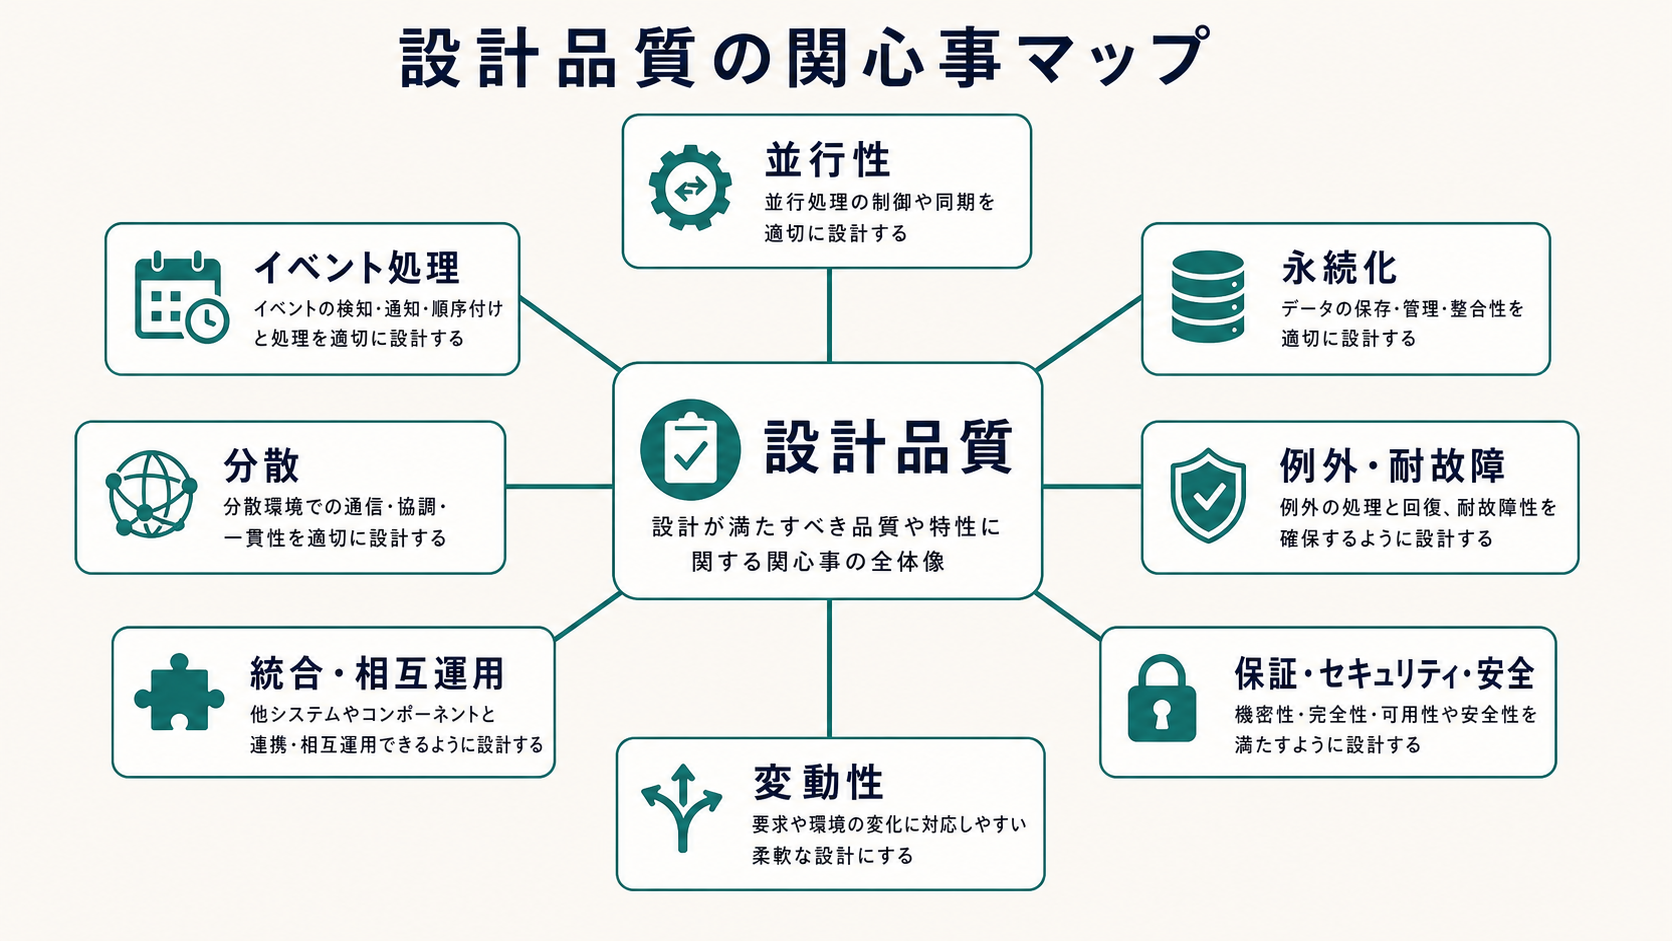
\includegraphics[width=0.96\linewidth]{assets/fig-ch03-06.png}}{\fbox{\parbox[c][48mm][c]{0.9\linewidth}{\centering 画像生成待ち\\設計品質の関心事マップ}}}
\caption{設計品質の関心事マップ}
\label{fig:ch03-06}
\end{figure}
